\subsection{BioPlex systematic AP-MS: co-complex check against the IntAct null}
\label{sec:bioplex}
The IntAct audit found no curated physical edge among the 21 AND-gate antigen
pairs, but curated resources can miss complexes that were never assayed at
small scale. BioPlex provides the orthogonal check: systematic affinity
purification--mass spectrometry networks over thousands of baits in two cell
lines (HEK293T 10K and HCT116 5.5K, Dec 2019 releases; 118,162 and
70,966 bait--prey edges). The limitation is complementary: a pair is
testable only when both antigens are expressed and detected in the cell line,
so BioPlex can confirm but not exhaustively exclude cis-complexes in
tumor-lineage contexts.

\paragraph{Calibration gate.} Pre-registered gates PASSED: (G1) PSMA1
recovers proteasome beta-subunit partners in both networks (observed
293T 8 PSMB partners, HCT116 9); (G2) POLR2A recovers at least one Pol~II subunit partner in
293T (observed POLR2D, POLR2E, POLR2F, POLR2G, POLR2J, POLR2L); (G3) at least three of four CAR-T reference
targets are detected in 293T (observed 4/4).

\paragraph{Antigen-pair co-complex test.} Of the 21 antigen pairs,
10 are testable in 293T and 6 in HCT116 (both antigens
detected). Observed co-precipitation edges: 0 in 293T and
0 in HCT116. CA9 and CLDN6 are undetected in both cell lines and
CLDN18 is undetected in HCT116, so pairs involving them remain untestable at
systematic scale. Three independent interaction screens (IntAct curation, BioPlex 293T, BioPlex HCT116) now agree: no physical co-complex is observed among testable AND-gate antigen pairs, so the two gate arms behave as independent surface targets on current evidence, bounded by the systematic-scale detection caveat above.

\paragraph{Detection and degree bias.} Gated genes are detected at higher
rates than background in both networks (72/99 versus 43/98 in 293T,
Fisher $p=4.86e-05$; 58/99 versus 28/98 in HCT116, $p=2.8e-05$),
so the gated set is well covered where it matters. Among detected genes,
however, AP-MS degree does NOT differ (medians 9.5 vs 10.0 in 293T,
$p=0.457$; 13.0 vs 8.5 in HCT116, $p=0.628$). The IntAct curated-degree advantage of the gated set (median 51 versus 15) therefore reflects study intensity rather than differential connectivity: measured systematically in a single experiment, gated and background genes are indistinguishable in AP-MS degree, and the higher gated detection rate makes the absence of antigen-pair edges the more credible.

\paragraph{Cross-resource concordance.} Restricting to universe--universe
pairs, BioPlex yields 38 edges in either network (6 reproduced
in both; cross-network Jaccard 0.16). All 38 BioPlex-either edges
are contained in the IntAct curated physical set (154 universe edges);
IntAct curates the BioPlex screens, so containment is expected by provenance
and serves as a mapping-validation anchor rather than independent evidence.
The 116 IntAct-only edges are small-scale curated evidence not
reproduced at systematic AP-MS scale in these two cell lines.

\begin{figure}[t]
\centering
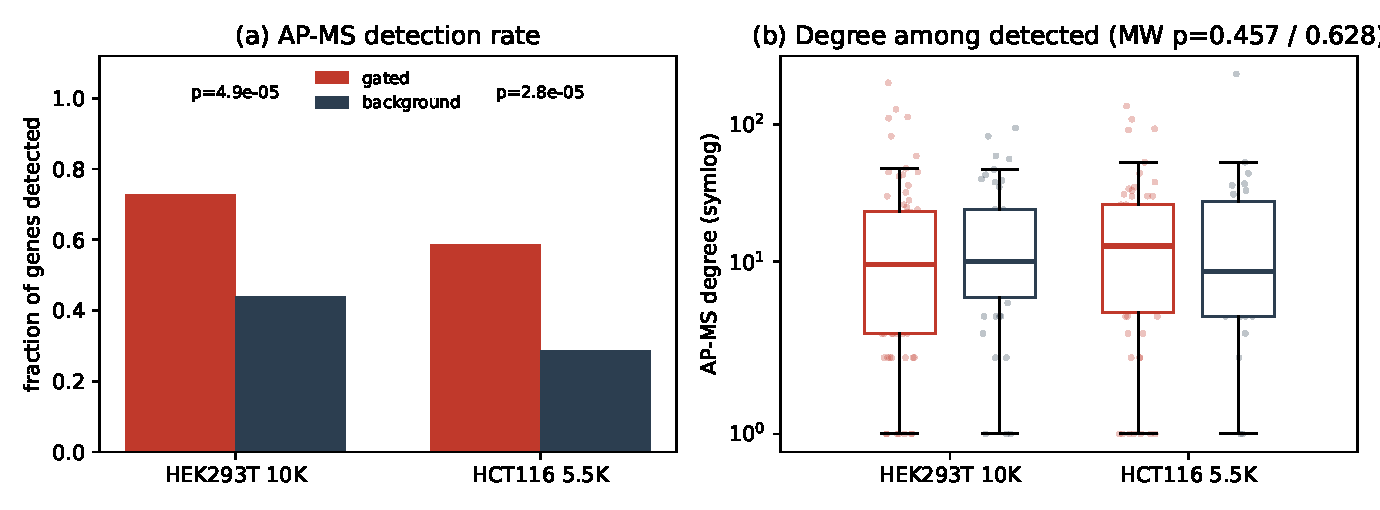
\includegraphics[width=\linewidth]{bioplex_fig.pdf}
\caption{BioPlex systematic AP-MS audit. (a) Detection rate of gated versus
background genes in the two networks. (b) AP-MS degree among detected genes
(symlog axis; boxes show median and quartiles).}
\label{fig:bioplex}
\end{figure}
